\documentclass[11pt]{article}
% Shared preamble. Deliberately built on stock `article` + widely-packaged dependencies rather than
% a venue .cls: the source has to compile for a reader who just cloned the repository, and swapping
% in acmart/neurips at submission time is a one-line change.

\usepackage[T1]{fontenc}
\usepackage[utf8]{inputenc}
\usepackage{lmodern}
\usepackage{microtype}
\usepackage[margin=1in]{geometry}
\usepackage{amsmath,amssymb}
\usepackage{booktabs}
\usepackage{array}
\usepackage{longtable}
\usepackage{graphicx}
\usepackage{xcolor}
\usepackage{caption}
\usepackage{subcaption}
\usepackage{listings}
\usepackage{enumitem}
\usepackage[hidelinks]{hyperref}
\usepackage[capitalise,noabbrev]{cleveref}
\usepackage{natbib}

\definecolor{codebg}{HTML}{F6F8FA}
\definecolor{rule}{HTML}{D0D7DE}
\definecolor{accent}{HTML}{1F4E79}

\captionsetup{font=small,labelfont=bf}
\setlist{itemsep=2pt,topsep=3pt,parsep=0pt}

\lstdefinestyle{policy}{
  basicstyle=\ttfamily\small,
  backgroundcolor=\color{codebg},
  frame=single,
  rulecolor=\color{rule},
  framesep=5pt,
  xleftmargin=6pt,
  breaklines=true,
  columns=fullflexible,
  keepspaces=true,
  showstringspaces=false,
}
\lstset{style=policy}

% Notation used throughout.
\newcommand{\Lpost}{\ensuremath{L^{\mathrm{post}}}}
\newcommand{\Rreg}{\ensuremath{\mathcal{R}}}
\newcommand{\headroom}{\ensuremath{H}}
\newcommand{\policyfam}{\ensuremath{\Theta}}
\newcommand{\shockstep}{\ensuremath{t^{\star}}}

% Data-dependent prose. Defaults say "pending" out loud, so a draft compiled before the sweep
% finishes announces that on the page instead of quietly reading as finished; the generated file
% \renewcommand's them once numbers exist.
\newcommand{\ResultsAbstractSentence}{\textcolor{red}{[results sentence pending the completed sweep]}}
\newcommand{\ResultsBody}{\textcolor{red}{[Results section pending the completed sweep. The tables
below are generated from the analysis artifact and are empty until it exists.]}}

% A boxed remark for the claims a reviewer will want to find quickly.
\newenvironment{takeaway}
  {\par\smallskip\noindent\begin{tabular}{@{}p{0.965\linewidth}@{}}\toprule\itshape}
  {\\\bottomrule\end{tabular}\par\smallskip}

\IfFileExists{generated/results_prose.tex}{% not enough results yet; the preamble's pending defaults stand.
}{}
\IfFileExists{generated/divergence_facts.tex}{% GENERATED by scripts/make_figures.py — do not edit.
\newcommand{\FrozenCost}{173.7}
\newcommand{\BestFixedCost}{170.0}
\newcommand{\SwitchCost}{123.5}
\newcommand{\DivergenceSeed}{0}
}{}
% Fallbacks so the document still compiles before the figure code has run.
\providecommand{\FrozenCost}{?}\providecommand{\BestFixedCost}{?}
\providecommand{\SwitchCost}{?}\providecommand{\DivergenceSeed}{?}
\providecommand{\MDEFraction}{?}

\title{\bfseries Rules That Stop Working\\
\large Why feedback institutions survive shocks to the world but not shocks to their own
instruments, and what it takes to notice}

\author{}
\date{}

\begin{document}
\maketitle

\begin{abstract}
\noindent
A standing policy rule---``restrict activity whenever the indicator crosses this threshold''---is a
feedback device, and feedback devices are unexpectedly robust. When the world worsens, the indicator
rises, the rule fires more often, and the institution keeps doing roughly the right thing without
anyone revisiting the statute. We show computationally that this robustness has a sharp boundary,
and that the boundary is not where the literature on institutional adaptation usually looks.

Using a simulated polity governing an endemic epidemic, we separate two kinds of structural break.
When the \emph{environment} changes---the pathogen becomes more transmissible---a rule calibrated
before the change remains within one percent of the best rule available after it. There is
essentially nothing for adaptation to do. When the \emph{instrument} changes---the same restriction
now delivers a quarter of the behavioural response while costing what it always cost---the pre-shock
rule carries a large excess burden, and its feedback structure makes matters worse rather than
better: rising prevalence causes it to intervene harder, buying less each time. The correct response
is not to stop governing but to \emph{substitute}: hold the instrument that still works and stop
paying for the one that broke.

We also show that what a stale rule costs \emph{factors}, into a part recoverable only by an
authority that notices and revises, and a part recoverable by having legislated a better rule in the
first place. The distinction has teeth: in two of the four polities we calibrate, the stale rule
costs $18$--$44\%$ while the adaptive part is worth nothing at all. An authority evaluated there
looks rigid while facing no adaptive problem, and the reform it would be prescribed---faster review,
more responsiveness, better monitoring---is the wrong one.

We then ask what an authority must be able to observe to notice. We give a policy-maker---instantiated
as a language model that writes its rules as short executable expressions, so that every enacted
policy is a legible, archivable artifact---a governing loop equipped with different informational
channels, and vary them factorially: a compliance channel reporting rule violations, a monitoring
channel reporting the realized performance of the policy actually in force, and an institutional
memory of precedents. \ResultsAbstractSentence

The design implication is specific. Auditing whether a rule was followed cannot reveal that the rule
has stopped working; only evaluating what the rule achieved can. Institutions built to detect
non-compliance are, in a precise and measurable sense, blind to instrument failure.
\end{abstract}

\section{The problem: when is a rule stale?}

Institutions govern through standing rules. A central bank follows a reaction function, a health
authority a threshold for restrictions, a regulator a trigger for intervention. Writing the rule
down is the point: it makes the state's behaviour predictable, reviewable, and contestable in a way
that discretionary case-by-case action is not.

The standard worry about such rules is that they go stale, and the canonical statement of the worry
is Lucas's: a relation estimated under one policy regime need not survive the introduction of
another \citep{lucas1976critique}, with Goodhart's \citeyearpar{goodhart1984monetary} corollary that
a measure targeted by policy ceases to be a good measure. Both are usually read as warnings about
\emph{estimation}. We want to read them as a question about \emph{institutional design}: given that
a rule will eventually stop working, what does the institution enforcing it have to be able to see
in order to find out?

This paper makes three moves. First, we show that ``the rule goes stale'' is far too coarse: the
staleness of a feedback rule depends on \emph{which part of the world moved}, and for one large
class of movements the rule barely goes stale at all. Second, we identify the class that does break
it---changes to the efficacy of the instrument the rule operates---and show why a feedback structure
converts that change from a nuisance into an active harm. Third, we vary the informational
architecture around a rule-writing authority and measure which channel is load-bearing for
detection.

\subsection{Why a computational model, and what it is for}

We use a simulation because the question is counterfactual in a way historical policy episodes
cannot be: we need to know how well the \emph{best available} rule would have performed after a
break in order to say whether an authority's response was good, and no observed polity provides
that. Our claim is not that the simulation predicts what any real health authority would do
\citep[a claim that would require far more than statistical realism;][]{li2026statistical}, but that
it isolates a mechanism and bounds it.

The policy-maker in our model is a large language model. We use it not as a claim about how humans
reason but as a convenient generator of \emph{written rules}: it must express its policy as a short
executable expression, which means every decision it takes leaves an inspectable artifact and its
revision history is measurable. Where prior work has language models set a tax rate or fill in a
fixed policy schema \citep{wang2025taxagent,li2023econagent,decurto2026narratives}, here the object
the authority produces is the rule itself. That is what makes questions like ``did the institution
revise its policy, and in which direction'' answerable at all.

\section{The model}
\label{sec:model-social}

A full ODD-style specification is in \cref{app:odd}; the essentials follow.

\paragraph{The governed system.} A population is partitioned into susceptible, infectious, and
recovered shares \citep{kermack1927contribution}. Immunity wanes and a small number of cases arrive
from outside, so the disease is \emph{endemic}: it does not burn out and cannot be waited out. This
is a substantive modelling choice rather than a technical one. In a model where the epidemic ends by
itself, ``do nothing until it is over'' is a viable strategy, and the interesting governance question
disappears.

\paragraph{The authority.} At regular review points the authority promulgates a standing rule
governing two costed instruments, restriction intensity and vaccination effort. The rule is applied
every period until replaced, not re-decided each period---an institution issuing a standing rule
rather than an administrator making daily calls. It is scored on infection burden plus a weight
$\lambda$ times intervention cost.

$\lambda$ is the polity's political economy in one number: the price it places on a unit of
restriction relative to a unit of illness. It is not a nuisance parameter to be marginalized. Set it
low and permanent maximal restriction is optimal; set it high and doing nothing is; and in both
cases the optimum sits at a corner where no shock can move it. Only at intermediate values does the
polity face a genuine trade-off, and only then can it be said to adapt at all. We report the whole
range (\cref{fig:surface}) rather than a single calibration.

\paragraph{The break.} At the midpoint of the horizon, without announcement, the efficacy of
restriction falls to a quarter: the same order produces a quarter of the behavioural change, while
costing exactly what it did before. Compliance fatigue is the obvious reading. Crucially,
\textbf{efficacy is never observable}. The authority sees prevalence, its own past choices, and
whatever its institutional memory retains. It never sees the parameter connecting them.

\section{Measuring what adaptation could be worth}
\label{sec:headroom-social}

Comparative claims about institutional adaptation are usually made against a single reference: the
policy that was in force before. That reference tells us whether an authority changed course
profitably. It cannot tell us whether changing course was worth much, and without that, a finding of
``no adaptation effect'' is uninterpretable---it may be a fact about the authority or a fact about
the situation.

We therefore calibrate two references inside one shared vocabulary of rules. The \emph{frozen} rule
is the best rule available given everything knowable before the break, held unchanged through it.
The \emph{clairvoyant} rule is the best rule in the same vocabulary given the break already known.
They differ in exactly one respect: when they were allowed to look. The ratio of their post-break
burdens is the \emph{adaptation headroom}, and it is the entire prize any adapting authority is
competing for.

\subsection{Two remedies, routinely conflated}
\label{sec:two-remedies}

One ratio is not enough, and the reason is a distinction with direct institutional consequences.
Write $\pi_{\mathrm{fixed}}$ for the best \emph{standing} rule over the whole broken horizon, chosen
with hindsight. Then what the stale rule costs factors:
\begin{equation}
\underbrace{\frac{L(\pi_{\mathrm{frozen}})}{L(\pi_{\mathrm{switch}})}}_{\text{staleness}}
=
\underbrace{\frac{L(\pi_{\mathrm{fixed}})}{L(\pi_{\mathrm{switch}})}}_{\text{adaptation headroom}}
\times
\underbrace{\frac{L(\pi_{\mathrm{frozen}})}{L(\pi_{\mathrm{fixed}})}}_{\text{robustness headroom}} .
\end{equation}

Staleness is the quantity the literature on institutional rigidity reports: the old rule is worse
now than it was. But it does not say what to do about it. The adaptation term is the part recoverable
\emph{only} by an authority that notices and revises. The robustness term is the part recoverable by
having written a different rule in the first place---by a legislature, not a regulator, and before
the fact rather than after.

We measure two cases where these separate completely, and they separate along different axes. Under
\emph{total} instrument failure at the baseline price, the stale rule costs $1.18\times$ and the
adaptation headroom is $1.01\times$. Holding the break at its baseline severity and raising the
\emph{price} of intervention instead, the stale rule costs $1.44\times$ and the adaptation headroom
is exactly $1.00\times$. In both, the best standing rule is effectively the same before and after
the break: nothing needed to change, the wrong rule had been written. An authority evaluated in
either would appear rigid while in fact facing no adaptive problem at all, and the reform it would
be prescribed---greater responsiveness, faster review cycles, better monitoring---would be the wrong
reform.

We report both because our first version varied severity and price \emph{together} and would have
credited the whole effect to severity. Separating them is what makes the claim a controlled one, and
it strengthened rather than weakened it: the finding holds along each axis by itself.

Notably, this is not what we expected. The severe regime was added on the assumption that a harsher
break leaves more for adaptation to recover. Measuring it says the opposite: past a point, the
failure is complete enough that a single robust rule dominates, and responsiveness buys nothing.

\begin{takeaway}
``This rule is costly'' and ``this rule must change'' are different diagnoses. Only the second is a
case for a more attentive government, and staleness alone cannot tell them apart.
\end{takeaway}

\begin{table}[t]\centering\small
\caption{\textbf{Decomposing what a stale rule costs.} All references are calibrated by
exhaustive search over the same policy vocabulary, on the same broken world, over the same seeds;
they differ only in what they were allowed to know. \emph{staleness}
$=L_{\text{frozen}}/L_{\text{switch}}$ is what the pre-break-optimal rule costs after the
break---the quantity a study of institutional rigidity usually reports, and on its own ambiguous.
It factors into \emph{adaptation headroom} $=L_{\text{fixed}}/L_{\text{switch}}$, the
part recoverable \emph{only} by changing behaviour mid-run, and \emph{robustness headroom}
$=L_{\text{frozen}}/L_{\text{fixed}}$, the part recoverable by having legislated a better
standing rule in the first place. The severe regime is the instructive case: a large staleness cost
with \emph{no} adaptation headroom at all. There the polity needed a better rule, not a more
attentive government---and reporting staleness alone would have called it an adaptation failure and
prescribed the wrong remedy.}
\label{tab:headroom}
\begin{tabular}{@{}l r r r r r r@{}}
\toprule
& \multicolumn{3}{c}{full-horizon loss} & \multicolumn{3}{c}{decomposition} \\
\cmidrule(lr){2-4} \cmidrule(lr){5-7}
regime & frozen & best fixed & switching & staleness & \textbf{adaptation} & robustness \\
\midrule
epidemic & 27.972 & 25.229 & 21.267 & 1.315 & \textbf{1.186} & 1.109 \\
epidemic\_pricey & 39.037 & 27.125 & 27.125 & 1.439 & \textbf{1.000} & 1.439 \\
epidemic\_severe & 29.967 & 25.648 & 25.482 & 1.176 & \textbf{1.007} & 1.168 \\
scalar & 0.036 & 0.033 & 0.032 & 1.125 & \textbf{1.039} & 1.083 \\
\bottomrule
\end{tabular}
\end{table}


\begin{figure}[t]\centering
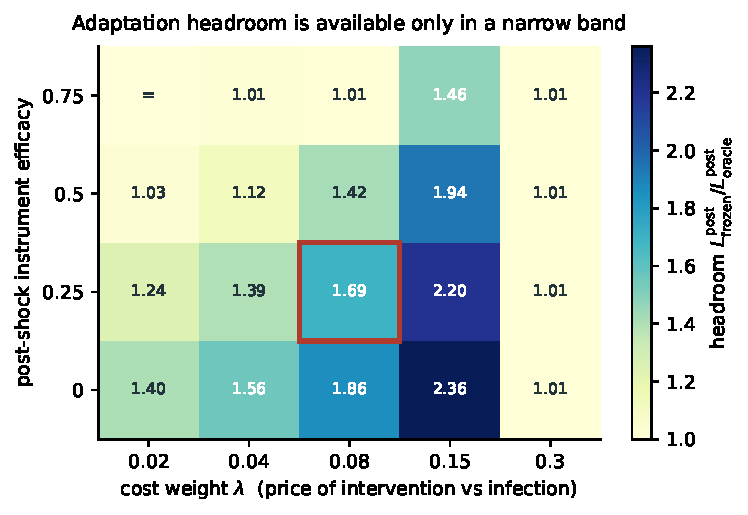
\includegraphics[width=0.82\linewidth]{generated/fig_headroom_surface}
\caption{\textbf{Adaptation is worth something only in a narrow band of political economies.}
Rows vary how badly the instrument fails; columns vary $\lambda$, the polity's price on
restriction. Cells marked ``='' are ones where the best rule before the break and the best rule
after it are \emph{the same rule}: the break does not move the optimum, so there is nothing to
adapt to. At low $\lambda$ the polity should always restrict and at high $\lambda$ never; both are
corner solutions and both are immune to the shock. Institutional adaptation is a meaningful category
only in between.}
\label{fig:surface}
\end{figure}

\subsection{The first result: which shocks a rule shrugs off}

\Cref{tab:headroom} and \cref{fig:surface} carry the paper's first finding. A shock to the
\emph{environment}---a more transmissible pathogen---leaves headroom of essentially one. The
pre-break rule remains near-optimal after the break, and no authority, however attentive, could have
demonstrated an improvement.

The reason is that a threshold rule is a feedback device. The shock raises prevalence; prevalence is
the variable the rule keys on; so the rule fires more often, entirely on its own. The institution
adapts without anyone adapting it, because the indicator still means what it meant.

A shock to the \emph{instrument} is different in kind. Nothing in the indicator reveals that a unit
of restriction now buys less, so no threshold on that indicator recovers the right behaviour. Worse,
the feedback structure that was protective before is now actively harmful: prevalence rises, so the
rule restricts harder, so the polity pays more for a fraction of the effect. The correct response is
to \emph{stop}, which is precisely the response the rule's own logic forbids.

\begin{takeaway}
Feedback rules are robust to shocks in the governed system and fragile to shocks in the governing
instrument. The robustness and the fragility have the same cause.
\end{takeaway}

\begin{figure}[t]\centering
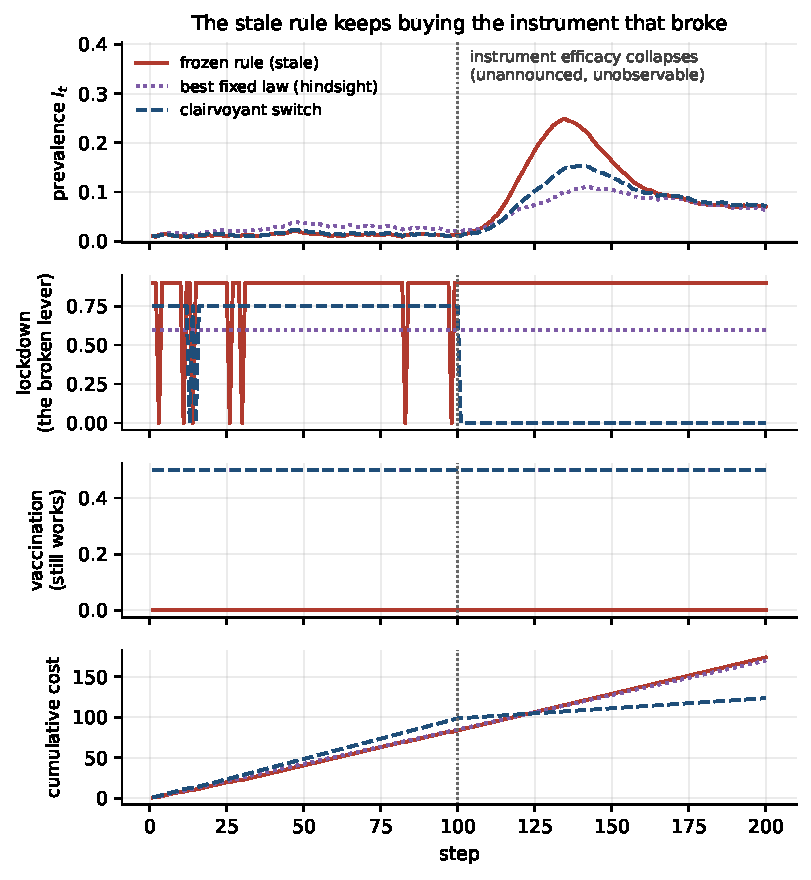
\includegraphics[width=0.72\linewidth]{generated/fig_policy_divergence}
\caption{\textbf{One polity, three institutions.} Before the break the frozen rule is the good
policy---it suppresses prevalence almost completely, which is why it was chosen. After the break it
continues to enact maximal restriction, accumulating cost while prevalence rises anyway. The
clairvoyant institution does not withdraw --- it \emph{substitutes}, holding vaccination at its
maximum throughout while dropping restriction to zero at the break. Cumulative cost on seed
\DivergenceSeed: frozen \FrozenCost, best fixed rule \BestFixedCost, clairvoyant \SwitchCost.
That distinction is the whole governance content of the figure: the right answer to an instrument
that stopped working is to reach for the one that still does, not to stop governing.}
\label{fig:divergence}
\end{figure}

\section{What must an institution see?}
\label{sec:channels-social}

If instrument failure is the case that matters, the design question becomes concrete: what
information does an authority need in order to detect one? We equip the rule-writing authority with
different channels and vary them factorially. Each is a recognizable piece of institutional
machinery:

\begin{description}[leftmargin=0em,style=nextline]
\item[Compliance reporting] The authority learns when its instructions were rejected or
malformed---the analogue of an enforcement or legal-validity channel. It reports on the
\emph{form} of the rule and says nothing about its consequences. An authority issuing valid rules
receives, correctly, no information from it at all.
\item[Outcome monitoring] The authority learns what its currently standing rule actually achieved
over the last review period, and retains the preceding entries. This is monitoring and evaluation in
the ordinary administrative sense. It is the only channel in which an unobservable instrument
failure leaves any trace, and the trace is indirect: two consecutive reviews reading ``same policy,
worse result''.
\item[Institutional memory] Retrieved precedent---the most similar past situations and what was done
then. Valuable for recurring problems and, across a structural break, potentially misleading, since
the most similar past situation may belong to a regime that no longer exists.
\end{description}

Stating the prediction in advance, and asymmetrically: monitoring should carry the effect;
compliance reporting should do nothing here; memory may be neutral or actively harmful across the
break. The full pre-registration, including the conditions under which we would withdraw rather than
adjust the claim, was committed before the treatment runs.

\section{Results}
\label{sec:results-social}

\ResultsBody

\begin{table}[t]\centering\small
\caption{\textbf{Full-horizon governance loss and normalized regret.} $\Rreg=1$ is the best
\emph{fixed} law in hindsight and $\Rreg=0$ the clairvoyant switch, so $\Rreg<1$ means the arm
did better than any standing rule could have---which, unlike a post-break-only comparison, passivity
alone cannot achieve. Lower is better; $\Rreg$ is computed per seed against the paired anchors
before averaging. $^{\dagger}$the critic arm is not budget-matched.}
\label{tab:arms}
\begin{tabular}{@{}l r r r r@{}}
\toprule
arm & $n$ & $L$ & sd & $\Rreg$ \\
\midrule
\textit{best fixed law in hindsight} & --- & 27.114 & --- & \textit{1.000} \\
\textit{clairvoyant switch} & --- & 23.736 & --- & \textit{0.000} \\
\midrule
no harness & 20 & 26.477 & 5.542 & \textbf{0.812} \\
trace & 20 & 26.477 & 5.542 & \textbf{0.812} \\
outcome & 20 & 26.475 & 5.257 & \textbf{0.811} \\
memory & 20 & 26.585 & 5.120 & \textbf{0.843} \\
\bottomrule
\end{tabular}
\end{table}

\begin{table}[t]\centering\small
\caption{\textbf{Factorial attribution of the harness.} $\pm1$ contrast coding with contrasts
formed within each seed, so world variance cancels. A \emph{negative} effect lowers post-break
loss, i.e.\ the component helped. Interactions are estimated, not assumed to be zero; $p$ is a
two-sided bootstrap value and $p_{\text{Holm}}$ corrects across the whole family of seven
terms.}
\label{tab:factorial}
\begin{tabular}{@{}l c r c r r c@{}}
\toprule
term & order & effect & 95\% CI & $p$ & $p_{\text{Holm}}$ & significant \\
\midrule
memory & 1 & +0.630 & $[+0.354, +0.901]$ & 0.0003 & 0.0021 & \textbf{yes} \\
outcome & 1 & +0.221 & $[-0.147, +0.595]$ & 0.2698 & 1.0000 & no \\
trace & 1 & -0.085 & $[-0.265, +0.034]$ & 0.4169 & 1.0000 & no \\
outcome:memory & 2 & -0.530 & $[-0.869, -0.180]$ & 0.0089 & 0.0534 & no \\
trace:outcome & 2 & -0.038 & $[-0.124, +0.035]$ & 0.3868 & 1.0000 & no \\
trace:memory & 2 & +0.038 & $[-0.049, +0.147]$ & 0.4914 & 1.0000 & no \\
trace:outcome:memory & 3 & -0.009 & $[-0.070, +0.055]$ & 0.7866 & 1.0000 & no \\
\bottomrule
\end{tabular}
\end{table}


\subsection{What the authority actually wrote}

Because policy here is code rather than a number, the enacted rules can simply be read.
\Cref{tab:crossmodel} reports whether the ordering replicates across the language models we could
access; more informative for a reader is the content of the rules themselves. Three observations
recur.

Authorities with no informational channel at all overwhelmingly emit \emph{constants}---a fixed
restriction level with no reference to the state of the epidemic. This is not a novel or creative
policy; it is a degenerate one, less responsive than the threshold rules the references use. An
authority with nothing to learn from does not merely fail to adapt: it never engages with the
situation in the first place.

Authorities with monitoring converge instead on \emph{proportional} rules, restricting in proportion
to prevalence. This form lies outside the threshold vocabulary the clairvoyant reference was
optimized within, which is a caution as much as a result---an authority that outperforms the
reference by writing a rule the reference could not express is telling us about our choice of
vocabulary. We therefore re-calibrate the clairvoyant reference over a widened vocabulary including
that form and report both comparisons.

Third, the direction of revision is measurable and it matters. An authority that responds to
worsening outcomes by restricting harder is failing in exactly the way the frozen rule fails, even
though it is nominally adapting.

\begin{table}[t]\centering\small
\caption{Cross-model replication.}\label{tab:crossmodel}
\emph{\textcolor{red}{Pending: the analysis artifact does not yet contain this table (cross\_model).}}
\end{table}


\section{Discussion}

\paragraph{An audit of compliance is not an audit of efficacy.} The sharpest implication is
negative. A channel that reports whether rules were followed contains no information about whether
following them still accomplishes anything. These are different questions, and an institution
equipped only for the first is blind to instrument failure by construction rather than by
inattention. That is a claim about informational architecture, and it does not depend on the
authority being a language model: any decision procedure restricted to compliance data faces the
same wall.

\paragraph{Rules fail in the direction of their own logic.} A feedback rule does not fail by going
quiet. It fails by doing more of what it does, more expensively, in response to the deterioration it
is itself failing to prevent. Escalation is the diagnostic signature of instrument failure, and it
looks from the inside exactly like the rule working hard.

\paragraph{Adaptation is a category with boundaries.} \Cref{fig:surface} shows that most of the
parameter space we might have studied contains no adaptation problem: at a corner solution the
optimal rule is invariant to the shock. This is worth stating to a literature that routinely asks
whether agents, institutions, or organizations adapt without establishing that adapting was
available. A null result in a region with no headroom is not evidence of rigidity.

\paragraph{Policy as a readable artifact.} Requiring the authority to express itself in code is a
methodological choice with a payoff for social science specifically: the object of study becomes a
sequence of legible rules with a revision history, rather than a sequence of actions from which a
rule must be inferred. Questions about \emph{how} policy changed---abruptly or gradually, in form or
in parameter, toward escalation or withdrawal---become directly measurable.

\section{Limitations}

The model is a stylized governance setting, not an epidemiological or public-health one, and nothing
here is a recommendation about restrictions. The authority is a language model, which is a
convenient rule-writer and not a model of human deliberation; we make no claim that its failures
resemble human ones. Model access was limited to what was reachable without paid inference, biasing
the panel toward smaller systems. Following \citet{ye2026trails} we audit robustness at the level of
the environment and the protocol but do not systematically vary the wording in which the authority's
task is described. Finally, in the present regime the clairvoyant response is close to withdrawal;
a stronger version, in which a second instrument survives the break so that the correct response is
substitution rather than retreat, is specified and not yet run.

\section{Conclusion}

Institutions do not usually fail because their rules were wrong when written. They fail because the
world moved and nothing in the institution's information flow made that visible. We have tried to
make that intuition precise: to separate the movements a feedback rule quietly absorbs from those it
converts into escalating harm, to measure how much any given movement leaves worth adapting to, and
to identify which of an institution's informational channels can carry the news. The channel that
can is the one that asks what the policy achieved. The channel that cannot---and that institutions
build first---is the one that asks whether the policy was obeyed.

\appendix
\section{Model specification (ODD-style)}
\label{app:odd}
\noindent Following the ODD convention, with the parameter values read directly from
the pinned configuration in \texttt{govsim/domains/scalar/regimes.py} rather than transcribed.

\subsection*{Purpose}
To determine which class of structural break a standing feedback rule can absorb, how much
adaptation is worth in each case, and which informational channel allows a rule-writing authority to
detect a break it cannot observe directly. The model is an instrument for isolating that mechanism;
it is not intended to forecast any real epidemic or to evaluate any real restriction policy.

\subsection*{Entities, state variables, and scales}
One governed population and one governing authority. The population is described by the shares
$S_t, I_t, R_t$ with $S+I+R=1$ enforced each step. The authority holds two instruments, restriction
intensity $\in [0, 0.9]$ and vaccination effort $\in [0, 0.5]$. One step is an epidemiological
period; the horizon is 200 steps and the authority reviews its rule every
10 steps, giving 20 reviews.

\subsection*{Process overview and scheduling}
Each step: (i)~the standing rule is re-evaluated against the current state and its output clipped
into the instrument's admissible range; (ii)~new infections, recoveries, vaccinations, and waning
are applied; (iii)~intervention cost accrues on the \emph{policy}, not on its effect. At a review
step the authority first receives whatever its channels supply, then promulgates a rule that stands
until the next review.

\subsection*{Design concepts}
\emph{Basic principle}: a standing rule is feedback, and feedback is robust to disturbances in
the signal it reads and fragile to changes in what its action accomplishes.
\emph{Adaptation}: the authority may rewrite its rule at review points; it is never told the
break occurred. \emph{Objective}: infection burden plus $\lambda=0.08$ times
intervention cost. \emph{Sensing}: $S, I, R$, the authority's own current instrument settings, and
the clock. Instrument efficacy is \textbf{never} sensed---inferring it is the task.
\emph{Stochasticity}: per-seed heterogeneity in $\beta_0$, $\gamma$, and initial prevalence,
plus per-step incidence noise. \emph{Observation}: the full trajectory, the enacted rules, and
every model call are recorded.

\subsection*{Initialisation}
$I_0 = 0.01$ with lognormal spread $\sigma=0.4$;
$\beta_0 = 0.35$ with lognormal spread $\sigma=0.18$;
$\gamma = 0.1$ with spread $\sigma=0.1$; $R_0 = 0$. Each of the 20
seeds draws one such population and every arm is run on all 20.

\subsection*{Input data}
None. The model is closed; no empirical time series is used as a driver.

\subsection*{Submodels}
\emph{Transmission}: $\beta_t = \beta_0\,(1 - a_t\,e_t)$, where $a_t$ is enacted restriction
and $e_t$ its efficacy. New infections are $\beta_t S_t I_t$ plus imported cases at rate
0.0005$\cdot S_t$ and Gaussian noise $\sigma=0.0015$, capped at $S_t$.
\emph{Recovery and waning}: a share $\gamma$ of $I$ recovers each step and a share
0.02 of $R$ returns to $S$, which makes the disease endemic---it cannot be waited out.
\emph{Vaccination}: moves $0.02\cdot v_t\, e^{\text{vac}}_t S_t$ from $S$ to
$R$. \emph{Cost}: $1.0\,a_t + 0.5\,v_t$ per step, charged on
the policy regardless of its effect---which is what makes an efficacy collapse expensive to ignore.
\emph{The break}: at $t = 100$, restriction efficacy
$e_t: 1.0 \to 0.25$. Transmissibility is unchanged
(\texttt{shock\_factor} $= 1.0$), so the break is purely
instrumental. It is not announced and leaves no directly observable trace.

\subsection*{Reference policies}
Calibrated by exhaustive search over 192 laws at
20 seeds:
frozen \texttt{0.9 if I > 0.01 else 0.0},
best fixed in hindsight \texttt{0.6 if I > 0.002 else 0.0}.


\section{Reproduction}
\label{app:repro-social}
\noindent Everything below is in the repository at commit \texttt{0ac002e-dirty}.

\begin{description}[leftmargin=0em,style=nextline]
\item[Calibrate the anchors] \texttt{uv run python scripts/recalibrate.py --seeds 20}
  \\writes \texttt{govsim/docs\_gates/calibration.json} (the artifact the paper's anchors are read from).
\item[Measure headroom across regimes] \texttt{uv run python scripts/headroom\_audit.py --seeds 8}
  \\and \texttt{scripts/decompose\_library.py --seeds 8} for the adaptation/robustness split.
\item[Run the matrix] \texttt{uv run python scripts/run\_matrix.py --arms epidemic --seeds 20 --store logs/runs\_v3}
  \\resumable: the model-call tape makes an interrupted sweep free to restart. Run \emph{one}
  sweep at a time --- the provider's binding quota is input tokens per minute, shared across
  processes, and concurrent sweeps exhaust the retry budget and kill an arm mid-run.
\item[Analyse] \texttt{uv run python scripts/analyze\_matrix.py --store logs/runs\_v3 --json logs/analysis\_v3.json}
\item[Regenerate these tables] \texttt{uv run python scripts/make\_tables.py --analysis logs/analysis\_v3.json}
\item[Replay without an API key] set \texttt{GOVSIM\_LLM\_MODE=replay}. Replay is served from a
  content-addressed tape keyed on the exact request, so a wrong key changes nothing and a missing
  entry raises rather than silently calling out. The tape for the reported runs is
  \textbf{39\,MB across 2913 files and is NOT committed to the repository}; export it from a
  completed store with \texttt{uv run python scripts/export\_tape.py --store logs/runs\_v3 --out logs/tape\_v3},
  or obtain it from the archived artifact. We state this plainly because the alternative --- claiming
  a committed tape that is not there --- is the kind of reproducibility promise that only fails once
  someone tries it.
\item[Tests] \texttt{uv run pytest} --- key-free, including the factorial estimator checked
  against data with a known generating effect.
\end{description}


\bibliographystyle{plainnat}
\bibliography{refs}

\end{document}
